\section{Results}
\label{sec:results}

We organize results by the five experiments: (1) synthetic Q/K stress test, (2) token-pattern stability in real attention, (3) end-to-end perplexity vs.\ \kvcache budget, (4) aggregation failure-mode probe, and (5) adaptive \kvcache quantization. Each tests a distinct facet of the hypothesis.

\subsection{Primitive validation on synthetic Q/K}
\label{sec:results:synth}

\para{Setup.} We plant token-conditioned attention structure: each of 100 vocabulary tokens has a fixed $(\vq, \vk)$ direction so that occurrences of the same token are designed to attend to overlapping positions. Sequence length $L = 512$, $H = 4$ heads, $d_h = 32$, three seeds. We sweep the storage threshold $\tau$ for \hma and compare to \streaming and \randomb at matched budget.

\para{Findings.} \tabref{tab:exp1} reports relative attention output error. At budget $\approx 16$, \hma's relative error is $\mathbf{98\times}$ lower than \randomb at the same budget (paired $t$-test $p < 10^{-4}$, $n = 3$ seeds). \streaming, despite a slightly larger budget, performs no better than random because the planted structure is global, not local. The lookup primitive captures the planted structure cleanly, validating the mechanism on data where token identity is a strong signal.

\begin{table}[h]
\centering
\caption{Synthetic Q/K stress test ($L = 512$, $H = 4$, $d_h = 32$, 3 seeds). \hma at small $\tau$ achieves near-zero error; \randomb and \streaming are essentially uninformative on globally token-conditioned data. Best in \textbf{bold}.}
\label{tab:exp1}
\begin{tabular}{@{}lcc@{}}
\toprule
\textbf{Method} & \textbf{Mean budget} & \textbf{Rel.\ attention error} \\
\midrule
\hma ($\tau=0.05$) & 15.2 & $0.013 \pm 0.000$ \\
\hma ($\tau=0.02$) & 15.7 & $0.005 \pm 0.000$ \\
\hma ($\tau=0.01$) & 16.1 & $0.003 \pm 0.000$ \\
\hma ($\tau=0.005$) & 16.5 & $0.001 \pm 0.000$ \\
\hma ($\tau=0.001$) & 17.5 & $\mathbf{0.000 \pm 0.000}$ \\
\streaming & 19.6 & $1.270 \pm 0.011$ \\
\randomb & 15.8 & $1.308 \pm 0.010$ \\
\bottomrule
\end{tabular}
\end{table}

\subsection{Token-pattern stability in GPT-2}
\label{sec:results:stability}

\para{Setup.} We run \gpttwo-small on a 1024-token \wikitext passage with full attention. For each query position, we take the top-16 attended keys and compute Jaccard overlap of these sets across query pairs grouped by (i) \emph{identity} (same token id), (ii) \emph{2-gram} (same last-two tokens), and (iii) \emph{distinct} (random pairs across distinct token ids).

\para{Findings.} \tabref{tab:exp2} shows the identity-versus-distinct lift is consistently positive across layers ($1.8{-}5.2\times$). 2-gram overlap exceeds identity at the deepest layer (0.210 vs.\ 0.176 at layer 11), supporting the user-proposed n-gram fuzzy lookup at deeper layers where context matters more than the token alone. Absolute Jaccard remains modest (0.1--0.2), indicating that the lookup alone will not reproduce full attention; sinks and a local window are still essential.

\begin{table}[h]
\centering
\caption{Top-16 attended-position Jaccard overlap on \gpttwo-small / \wikitext, by query-pair grouping. Identity is consistently $1.8{-}5.2\times$ higher than distinct; 2-gram overtakes identity at layer 11, suggesting context matters more in deeper layers.}
\label{tab:exp2}
\begin{tabular}{@{}lcccc@{}}
\toprule
\textbf{Layer} & \textbf{identity} & \textbf{2-gram} & \textbf{distinct} & \textbf{identity / distinct} \\
\midrule
0  & 0.089 & 0.079 & 0.017 & $5.16\times$ \\
6  & 0.091 & 0.088 & 0.050 & $1.84\times$ \\
11 & \textbf{0.176} & \textbf{0.210} & 0.074 & $2.39\times$ \\
\bottomrule
\end{tabular}
\end{table}

\subsection{End-to-end perplexity vs.\ KV budget}
\label{sec:results:ppl}

\para{Setup.} A 512-token \wikitext passage with prefill on the first 256 tokens and decode-region NLL on the next 256 (full-attention oracle perplexity 22.43). We sweep target budget $b \in \{32, 64, 128, 256\}$ for each method. Effective budget reports the mean candidate-set size at decode time; for threshold-based \hma, this is often \emph{smaller} than the cap because the stored set saturates.

\para{Findings.} \tabref{tab:exp3} summarizes the budget--perplexity trade-off. \figref{fig:ppl_vs_budget} visualizes the same data. Three observations:

\begin{itemize}[leftmargin=*,itemsep=0pt,topsep=0pt]
    \item \hma dramatically beats \randomb and a windowless \hto at every budget (\eg 90.6 vs.\ 2972 vs.\ 399 at budget $\approx 32$). The published \hto includes a sliding-window component that we did not stack in this comparison; our \hto numbers should be read as a heavy-hitter \emph{ablation}, not as a full reproduction of \hto.
    \item At small budgets, \hmaid edges out \streaming: at effective budget 24.8 \hmaid reaches \ppl 90.6 vs.\ \streaming's \ppl 95.7 at budget 32 --- about 22\% smaller effective \kvcache for similar quality.
    \item At larger budgets, \streaming and \hma converge; \hmang eventually edges out \streaming (\ppl 37.6 vs.\ \streaming's 30.2 at $b = 256$, \ie still slightly higher) but the gap is small. The most honest reading is that \hma matches a well-tuned \streaming baseline, with a measurable advantage only at small budgets.
    \item \hma's effective budget is sublinear in $b$: at cap 256, the stored set saturates at $\approx 133$, suggesting the underlying attention is genuinely sparse and the cap is mostly redundant.
\end{itemize}

\begin{table}[h]
\centering
\caption{\wikitext perplexity vs.\ \kvcache budget on \gpttwo-small ($L=512$, prefill$=256$, decode$=256$). Best (lowest) at each effective budget tier in \textbf{bold}. Full-attention oracle perplexity is 22.43.}
\label{tab:exp3}
\begin{tabular}{@{}lccc@{}}
\toprule
\textbf{Method} & \textbf{Target budget} & \textbf{Effective budget} & \textbf{Perplexity} \\
\midrule
\full & --- & 384 & \textbf{22.43} \\
\midrule
\streaming & 32 & 32.0 & 95.68 \\
\randomb & 32 & 32.0 & 2972.17 \\
\hto & 32 & 32.0 & 399.18 \\
\hmaid & 32 & 24.8 & \textbf{90.64} \\
\midrule
\streaming & 64 & 64.0 & 54.30 \\
\hmaid & 64 & 44.2 & \textbf{59.97} \\
\midrule
\streaming & 128 & 128.0 & \textbf{43.66} \\
\randomb & 128 & 128.0 & 300.51 \\
\hto & 128 & 128.0 & 448.16 \\
\hmaid & 128 & 79.1 & 49.07 \\
\hmang & 128 & 69.3 & 45.82 \\
\midrule
\streaming & 256 & 256.0 & \textbf{30.22} \\
\hmang & 256 & 133.2 & 37.61 \\
\bottomrule
\end{tabular}
\end{table}

\begin{figure}[h]
\centering
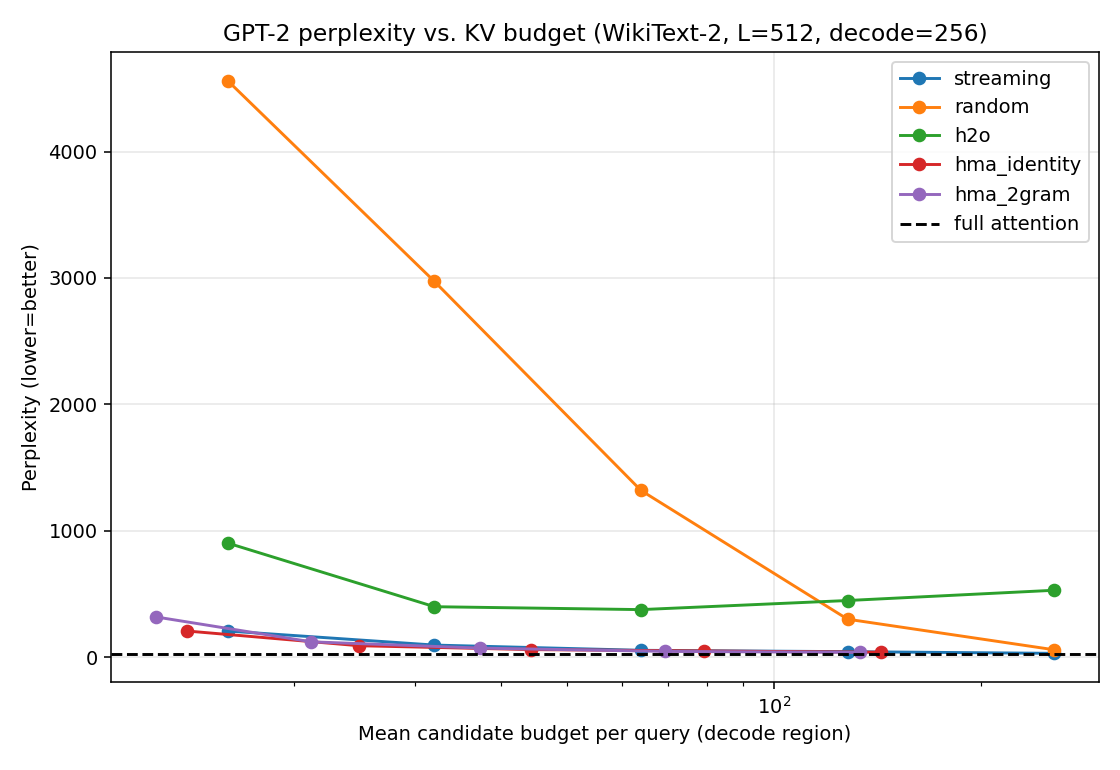
\includegraphics[width=0.7\linewidth]{figures/exp3_ppl_vs_budget.png}
\caption{\wikitext perplexity vs.\ effective \kvcache budget on \gpttwo-small. \hma (red) tracks \streaming (blue) closely and edges below it at small budgets; \randomb and windowless \hto are off the scale. Lower is better.}
\label{fig:ppl_vs_budget}
\end{figure}

\subsection{Aggregation failure-mode probe}
\label{sec:results:agg}

\para{Setup.} \magicpig \citep{chen2024magicpig} showed that LSH-Top-K methods collapse on aggregation tasks (\ruler-cwe/fwe) because Top-K cannot capture the broad attention pattern required to count or average over many positions. We construct a small synthetic ``common-word counting'' probe: a query token is a target word, and the correct attention output is an average over \texttt{target\_freq} other positions of the same word. We measure \hma's relative error at the final query as \texttt{target\_freq} grows from 1 to 64. Five seeds.

\para{Findings.} \tabref{tab:exp5} shows \hma's candidate set scales naturally from 13 to 41 candidates as target frequency grows from 1 to 64, with relative error remaining $\leq 0.013$. Threshold-based storage (\ie ``store all positions with weight $> \tau$'') is a non-Top-K rule and consequently does not exhibit the Top-K aggregation collapse that strict $k$-best selection would. This is direct empirical evidence that \hma sidesteps the failure mode \magicpig identified.

\begin{table}[h]
\centering
\caption{Aggregation probe: \hma relative error and candidate count as the target word's frequency grows. The candidate set scales with frequency; relative error stays small. Threshold-based storage avoids the Top-K aggregation collapse.}
\label{tab:exp5}
\begin{tabular}{@{}cccc@{}}
\toprule
\textbf{Target freq} & \textbf{Mean target count} & \textbf{HMA candidates} & \textbf{Rel.\ error} \\
\midrule
1  & 2.0  & 13.0 & $0.003 \pm 0.004$ \\
4  & 4.8  & 15.6 & $0.001 \pm 0.001$ \\
16 & 15.6 & 23.8 & $0.003 \pm 0.001$ \\
32 & 28.2 & 32.4 & $0.007 \pm 0.002$ \\
64 & 43.0 & 40.8 & $0.013 \pm 0.002$ \\
\bottomrule
\end{tabular}
\end{table}

\subsection{Adaptive KV quantization}
\label{sec:results:quant}

\para{Setup.} We assign per-(layer, head, position) bit-widths driven by hit count $c_j^{(\ell, h)}$, computed during a full-attention pass. We compare to (i) uniform quantization at $\{2, 3, 4, 6, 8\}$ bits, and (ii) random allocation at the same fractions but with positions assigned uniformly at random. Full-precision perplexity is 25.14.

\para{Findings.} \tabref{tab:exp6} and \figref{fig:quant} show:
\begin{itemize}[leftmargin=*,itemsep=0pt,topsep=0pt]
    \item Uniform 6- and 8-bit quantization is essentially lossless for \gpttwo's \kvcache; quantization loss appears at 4 bits and below.
    \item \emph{Adaptive at $\bar{b} = 3.90$ bits beats uniform 4-bit at lower memory} (\ppl 26.41 vs.\ 27.34), a clean Pareto improvement.
    \item Adaptive consistently beats random at every matched bit-budget (26.41 vs.\ 27.12 at $\bar{b} = 3.90$; 25.14 vs.\ 25.40 at $\bar{b} = 6.00$), confirming that hit count is informative for bit allocation.
    \item At $\bar{b} = 6.00$ the adaptive policy matches full-precision perplexity exactly.
\end{itemize}
This validates the second arm of the user's hypothesis: \hma's hit-count signal is a useful complement to existing per-channel/per-token \kvcache quantization schemes.

\begin{table}[h]
\centering
\caption{\kvcache quantization on \gpttwo-small / \wikitext (full-precision \ppl 25.14). Adaptive at $\bar{b} = 3.90$ bits beats uniform 4-bit at lower memory, and consistently beats random allocation at matched fractions. Best at each $\bar{b}$ tier in \textbf{bold}.}
\label{tab:exp6}
\begin{tabular}{@{}lcc@{}}
\toprule
\textbf{Method} & \textbf{Avg bits} & \textbf{Perplexity} \\
\midrule
\full (FP32) & 32.0 & 25.14 \\
\midrule
Uniform 8-bit & 8.0 & 25.16 \\
Uniform 6-bit & 6.0 & 25.17 \\
Uniform 4-bit & 4.0 & 27.34 \\
Uniform 3-bit & 3.0 & 46.83 \\
Uniform 2-bit & 2.0 & 290.53 \\
\midrule
Adaptive (50/50: 8b/4b) & 6.00 & \textbf{25.14} \\
Adaptive (25/75: 8b/4b) & 5.00 & \textbf{25.37} \\
Adaptive (10/90: 8b/4b) & 4.40 & \textbf{25.68} \\
Adaptive (10/40/50: 8b/4b/3b) & 3.90 & \textbf{26.41} \\
\midrule
Random (50/50: 8b/4b) & 6.00 & 25.40 \\
Random (10/40/50: 8b/4b/3b) & 3.90 & 27.12 \\
\bottomrule
\end{tabular}
\end{table}

\begin{figure}[h]
\centering
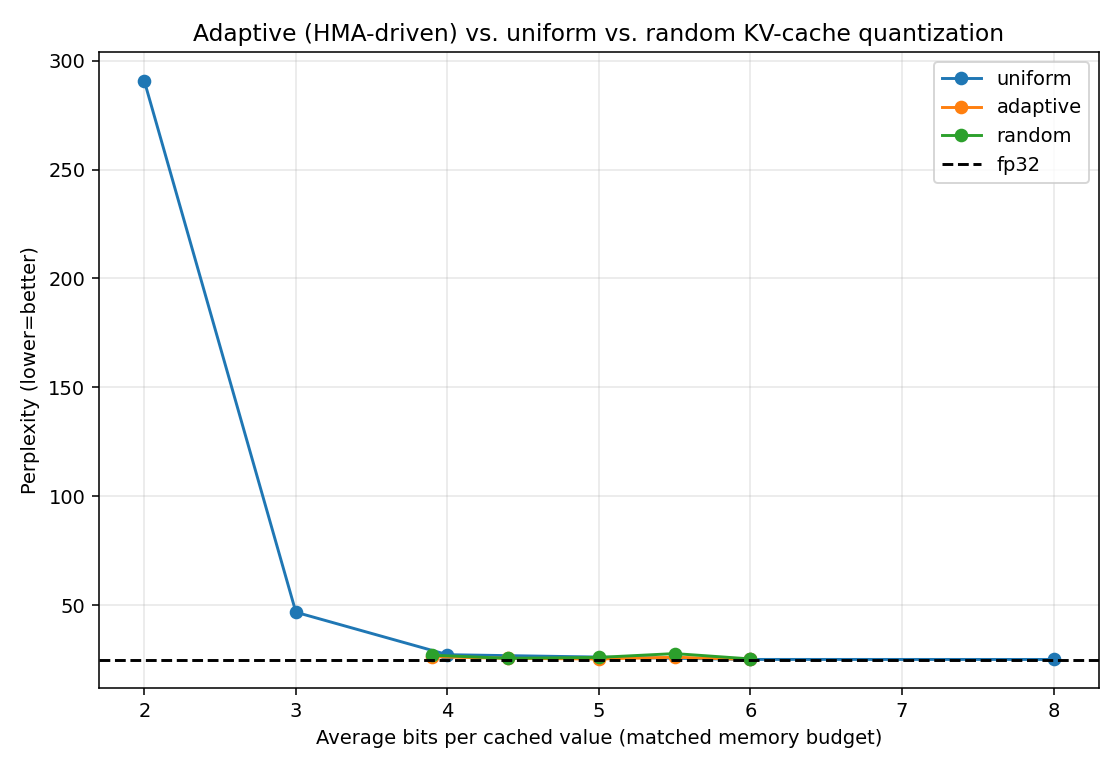
\includegraphics[width=0.7\linewidth]{figures/exp6_quant.png}
\caption{Pareto curve for \kvcache quantization on \gpttwo-small. Adaptive (\hmaquant) lies below the uniform and random curves: at 3.9 average bits adaptive achieves \ppl 26.4 vs.\ uniform 4-bit's 27.3 at strictly higher memory. Lower-left is better.}
\label{fig:quant}
\end{figure}

\subsection{Ancillary plots}
\label{sec:results:plots}

\figref{fig:budget_error}, \figref{fig:jaccard}, and \figref{fig:agg} present the corresponding visualizations for experiments 1, 2, and 5.

\begin{figure}[h]
\centering
\begin{subfigure}[b]{0.32\textwidth}
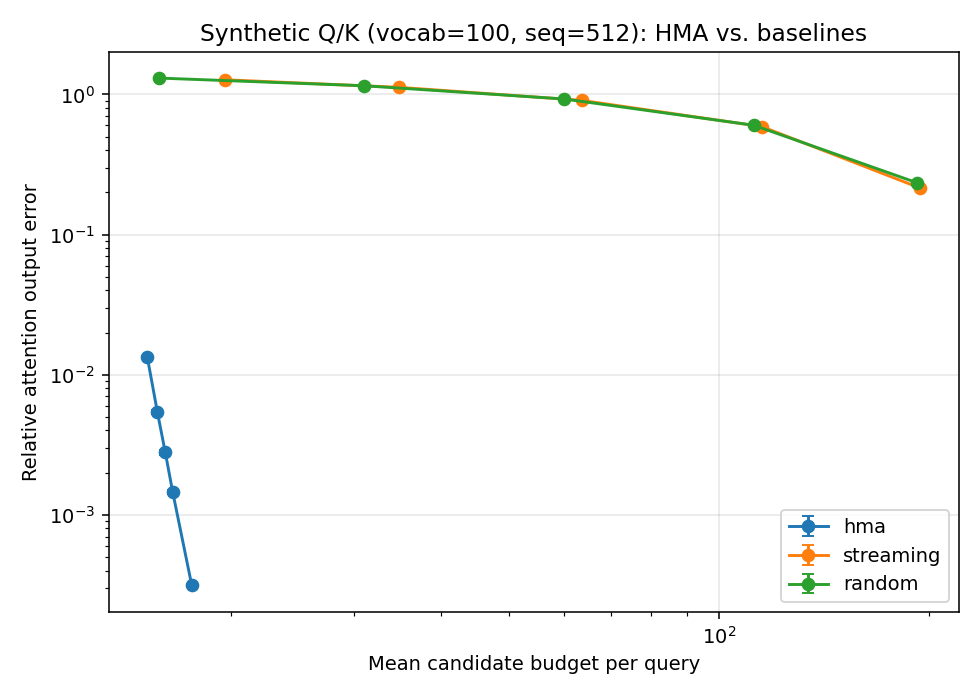
\includegraphics[width=\textwidth]{figures/exp1_budget_vs_error.png}
\caption{Synthetic Q/K stress.}
\label{fig:budget_error}
\end{subfigure}
\begin{subfigure}[b]{0.32\textwidth}
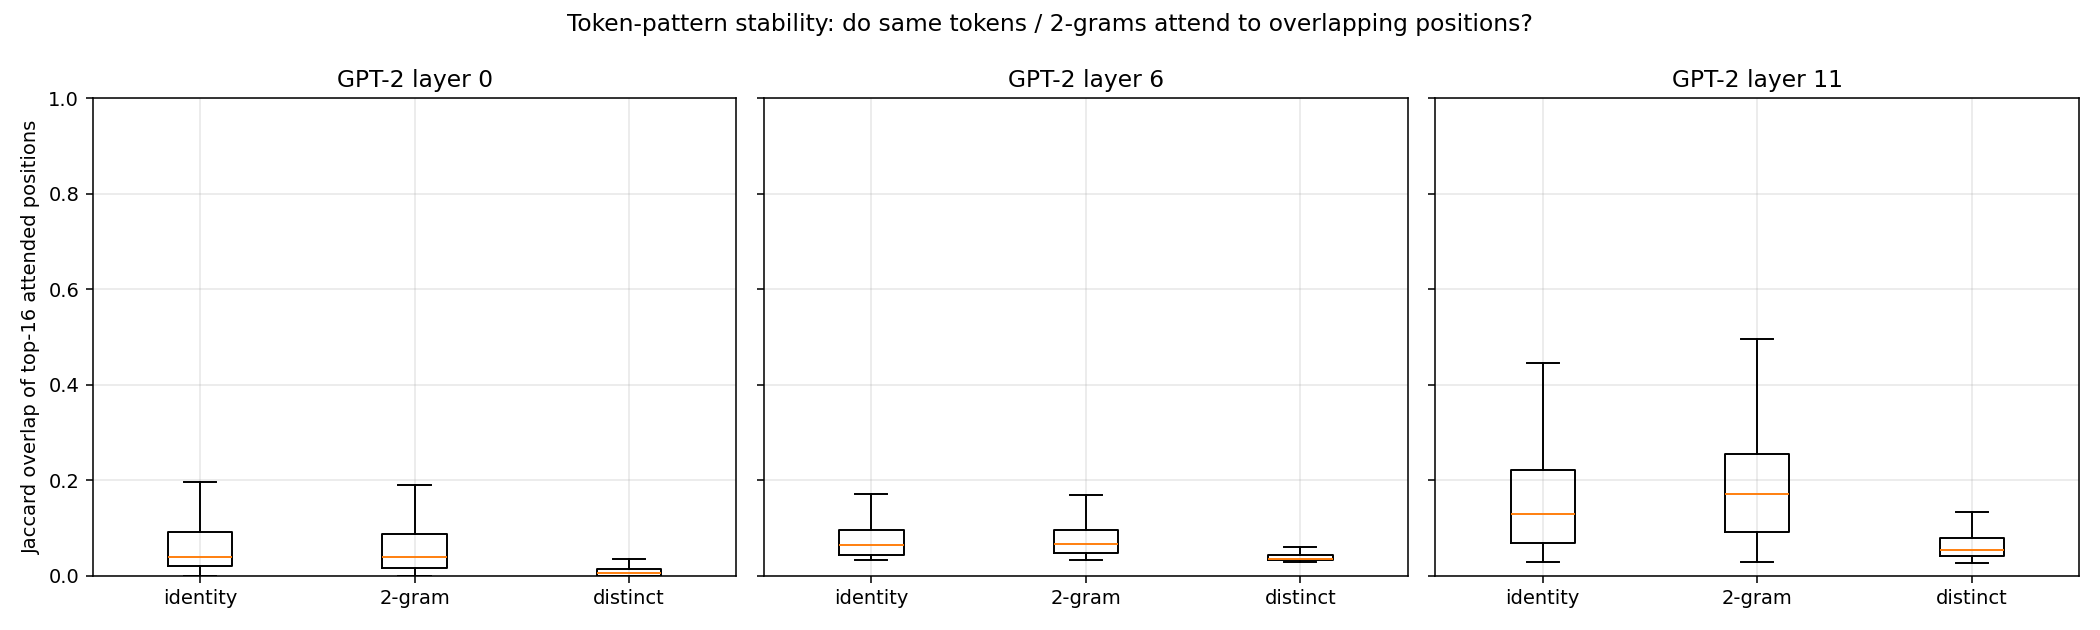
\includegraphics[width=\textwidth]{figures/exp2_jaccard.png}
\caption{Jaccard by layer.}
\label{fig:jaccard}
\end{subfigure}
\begin{subfigure}[b]{0.32\textwidth}
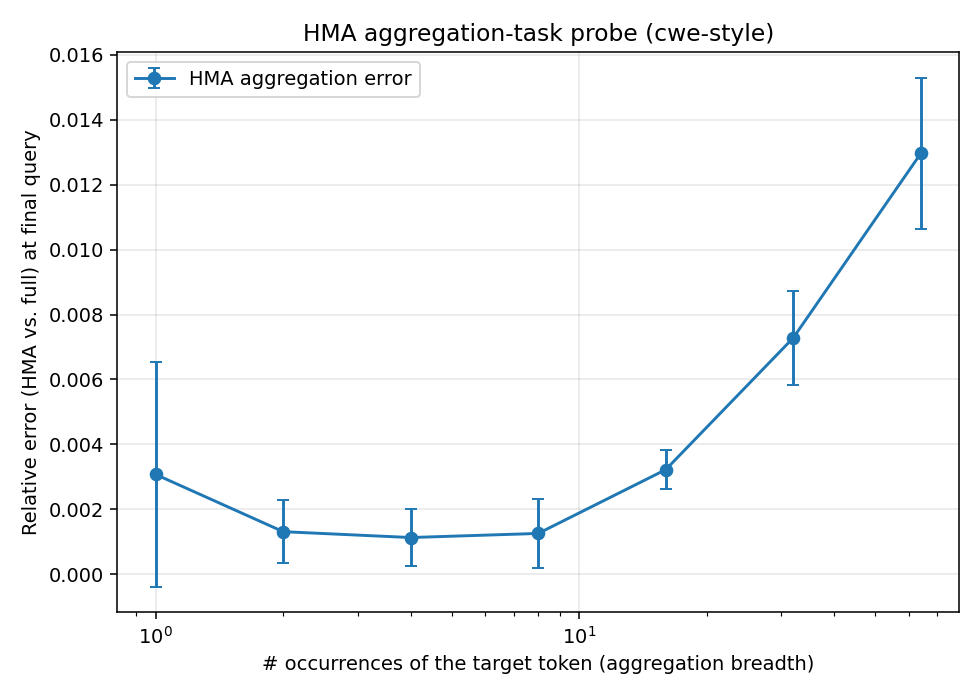
\includegraphics[width=\textwidth]{figures/exp5_aggregation.png}
\caption{Aggregation probe.}
\label{fig:agg}
\end{subfigure}
\caption{\figleft Budget vs.\ relative attention error on planted Q/K data; \hma is multiple orders of magnitude below random and streaming. \figcenter Top-16 Jaccard overlap by layer for identity, 2-gram, and distinct query pairs on \gpttwo-small. \figright Aggregation probe: \hma candidate count and relative error vs.\ target frequency.}
\label{fig:ancillary}
\end{figure}
